\begin{posterblock}{white}{smured}{smugold}{smucream!70}{R2. Results: AE Activity and Assembly Integrity Checks}
\begin{columns}[t,totalwidth=\linewidth]
\begin{column}{0.34\linewidth}
\centering
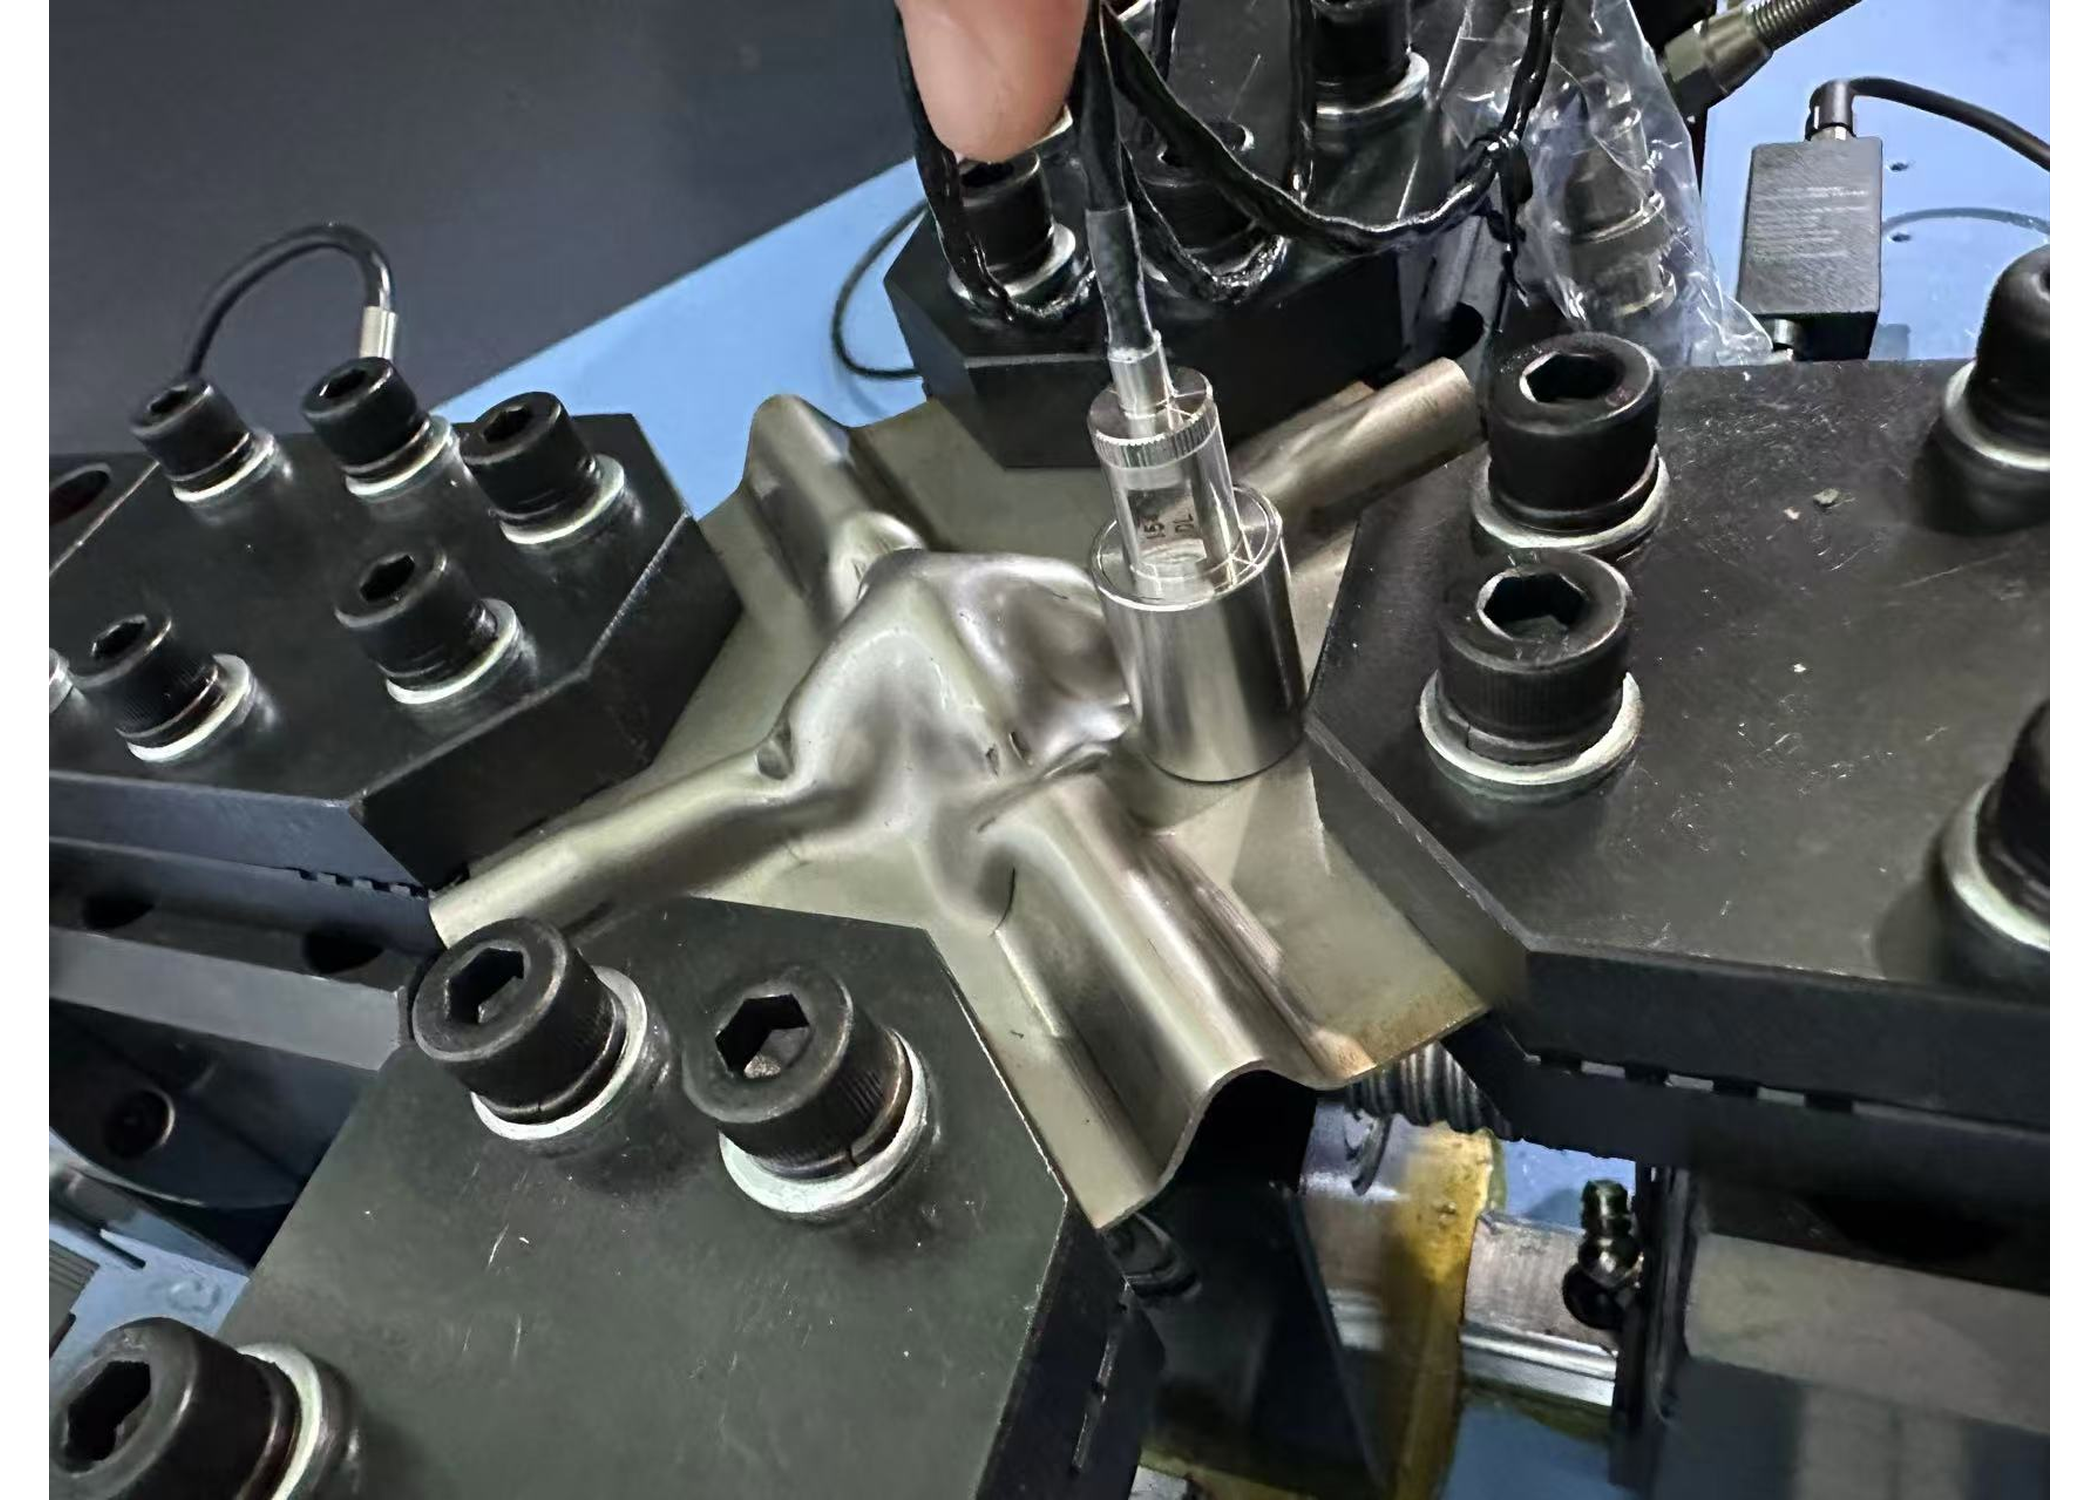
\includegraphics[width=\linewidth]{assets/fig04a_uploaded_ae_sensor_installation_photo.png}
\smallnote{AE sensors were mounted during the same four-axis loading context.}
\end{column}
\hfill
\begin{column}{0.62\linewidth}
\compacttable
\renewcommand{\arraystretch}{1.12}
\begin{tabular}{@{}>{\bfseries}p{0.25\linewidth}p{0.60\linewidth}@{}}
\toprule
Rule & Interpretive use \\
\midrule
Relabel cycles & PLC peak counting resets the AE coordinate before interpretation. \\
Track features & amplitude, high-amplitude fraction, and energy indicate cyclic activity. \\
Keep boundary & feature trends screen damage evolution; they do not alone prove cracks. \\
\bottomrule
\end{tabular}
\end{column}
\end{columns}

\centering
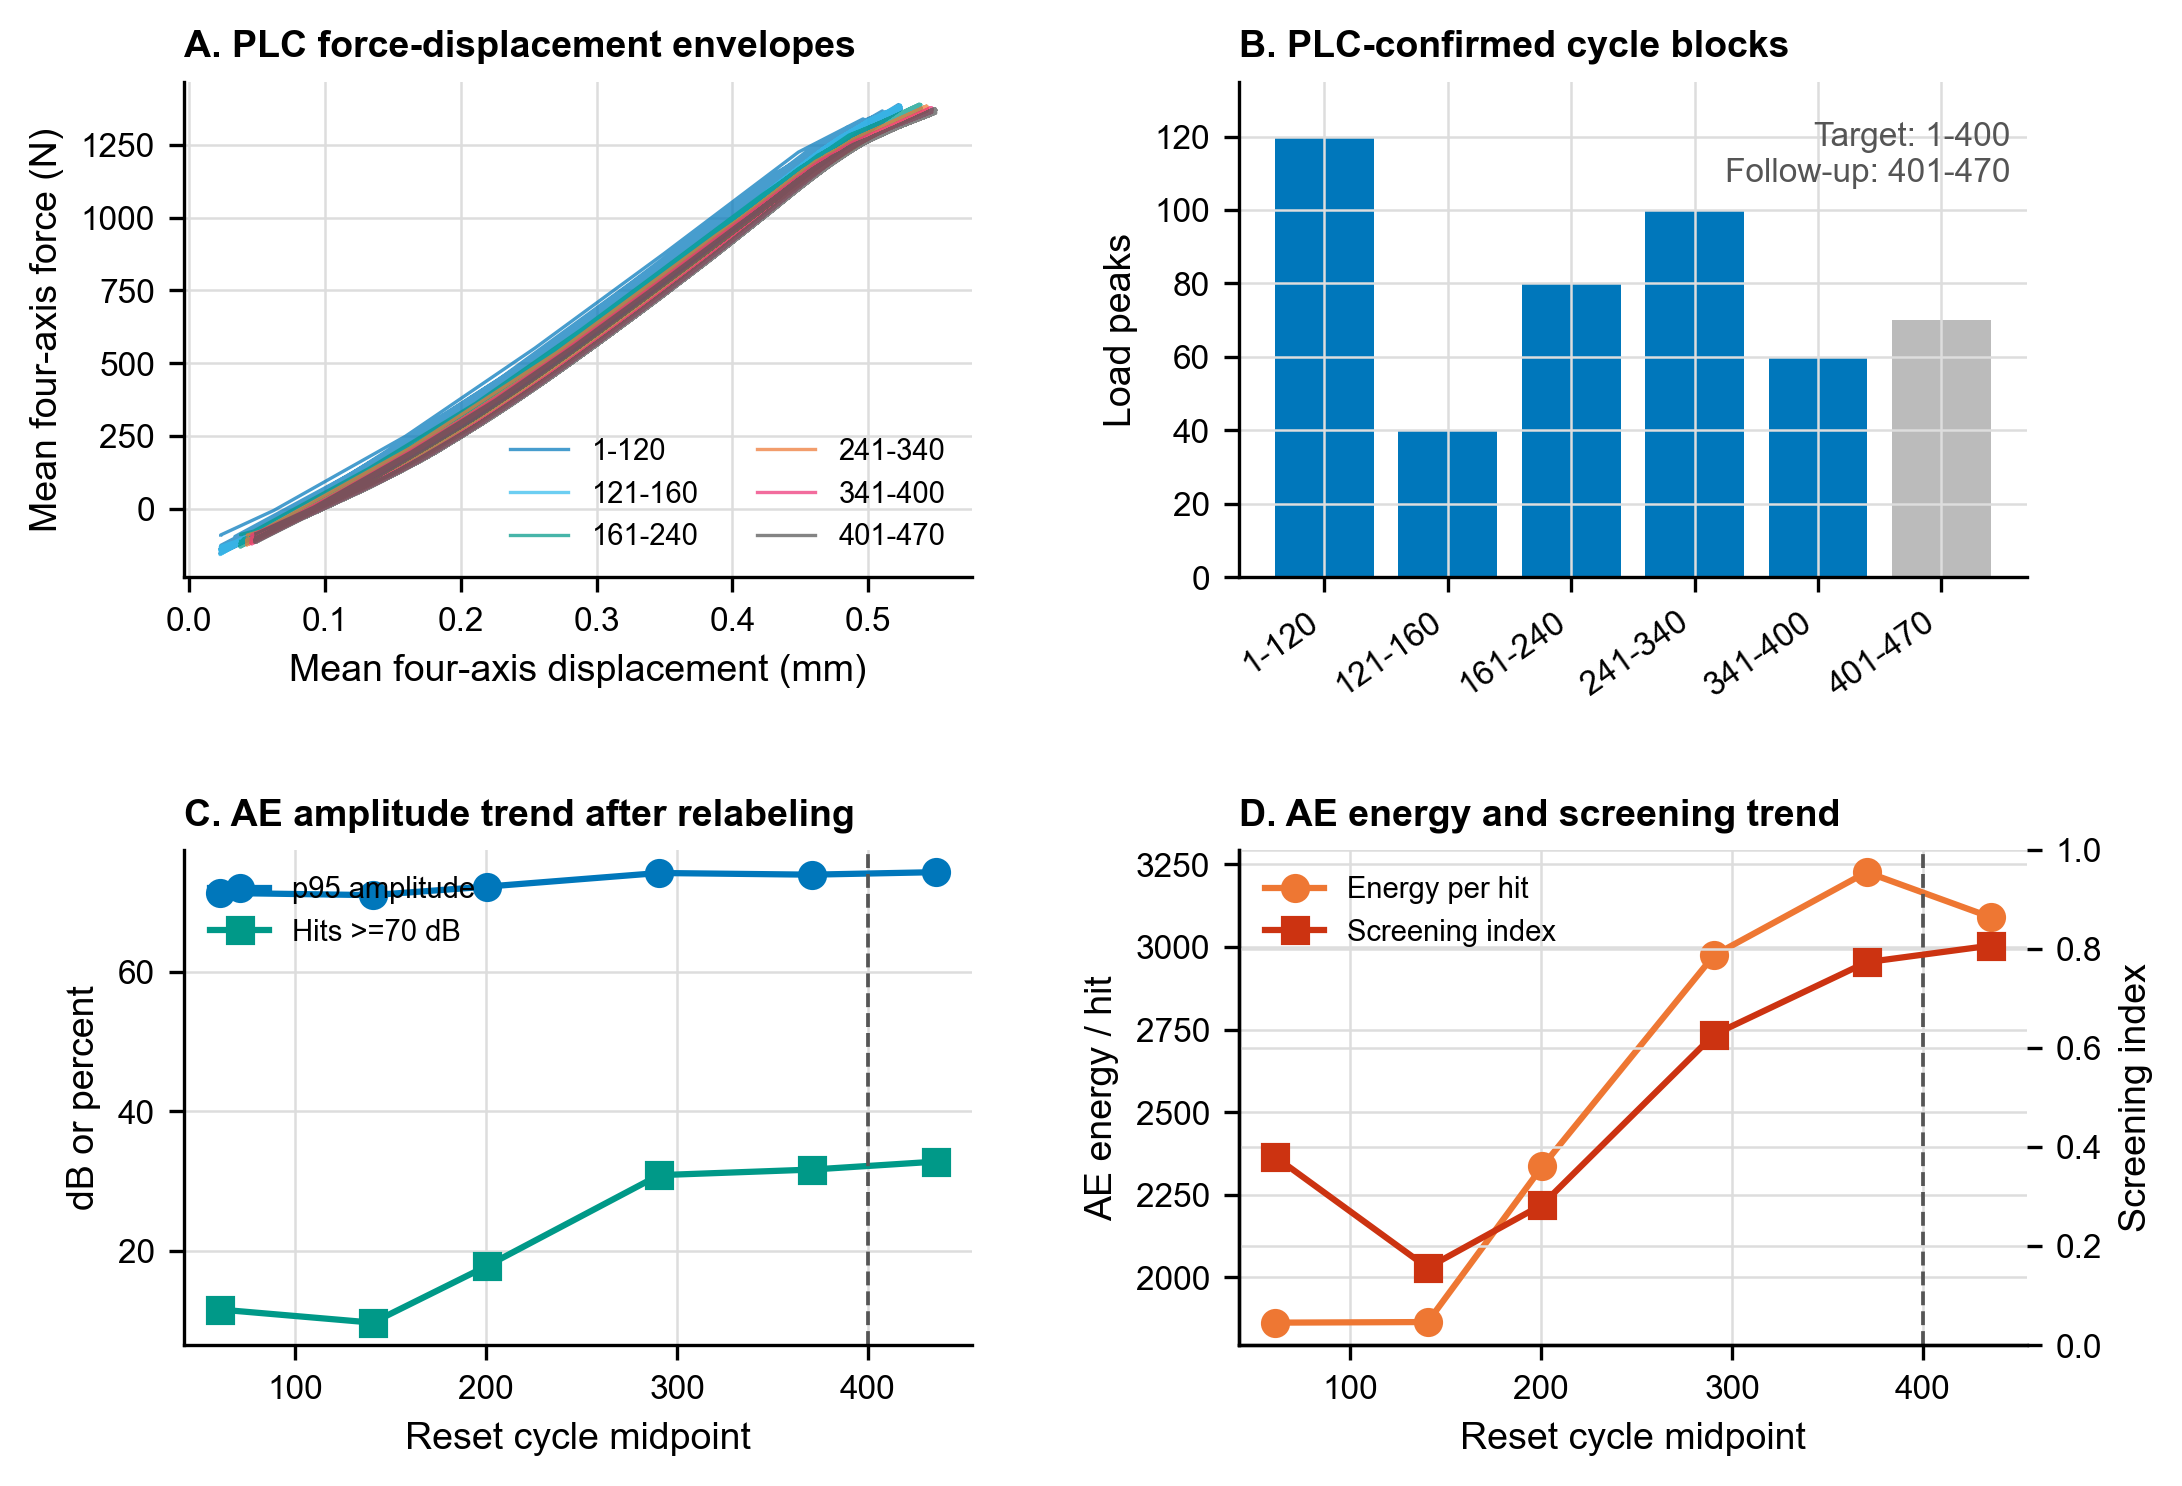
\includegraphics[width=\linewidth]{assets/fig04b_ae_cyclic_force_alignment.png}
\smallnote{PLC peak counting defines reset cycles 1--400 and follow-up 401--470.}

\vspace{0.65ex}
\centering
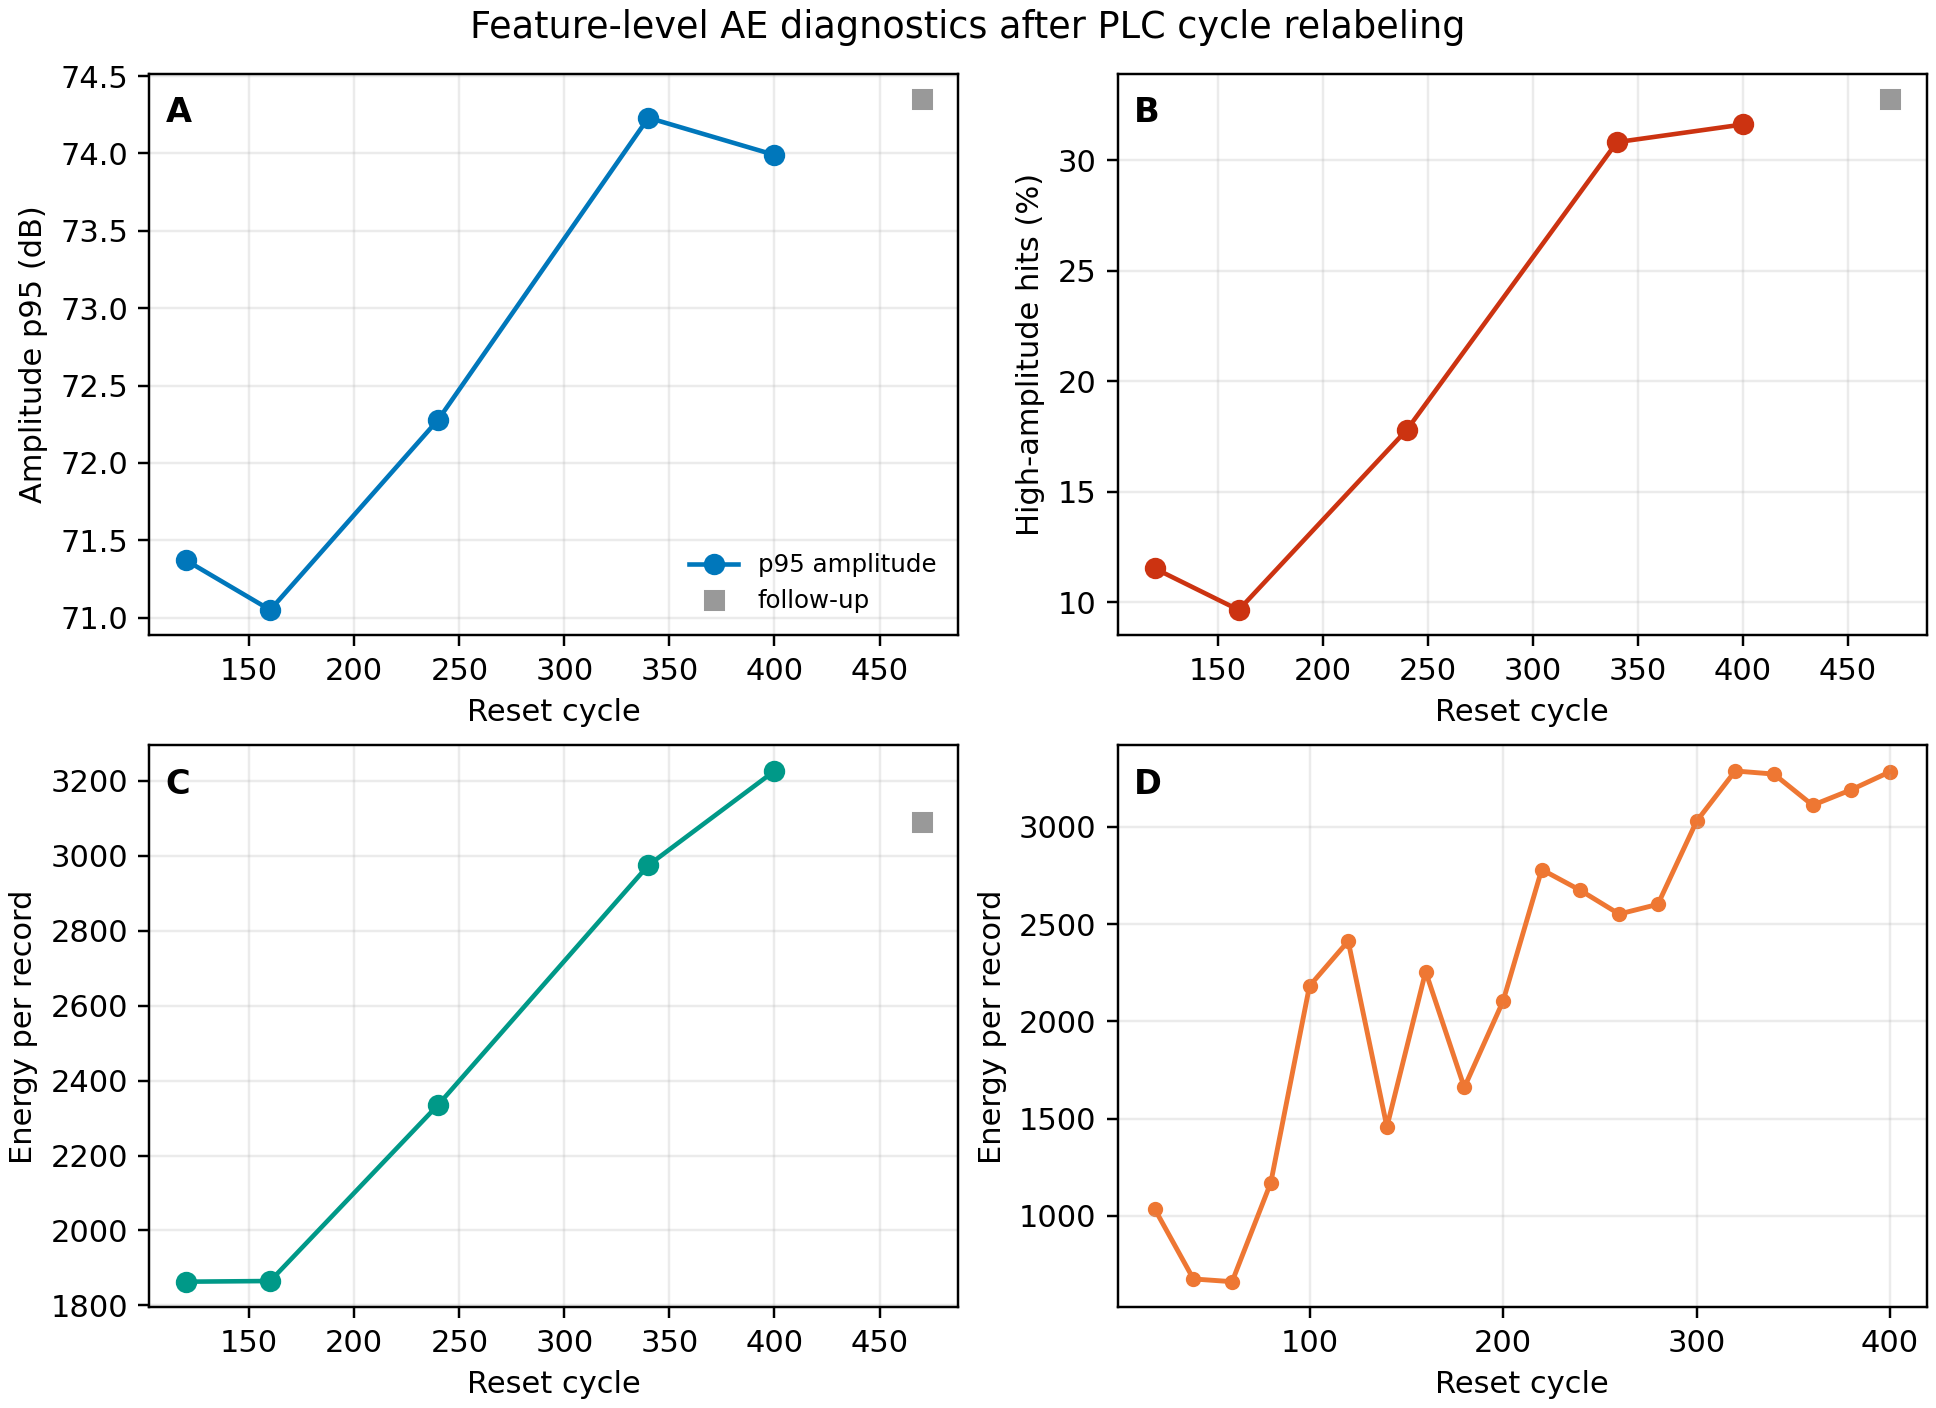
\includegraphics[width=\linewidth]{assets/fig04c_ae_full_feature_diagnostics.png}
\smallnote{Damage-evolution screen: p95 amplitude, high-amplitude fraction, and energy increase toward the late reset-cycle window.}

\vspace{0.65ex}
\centering
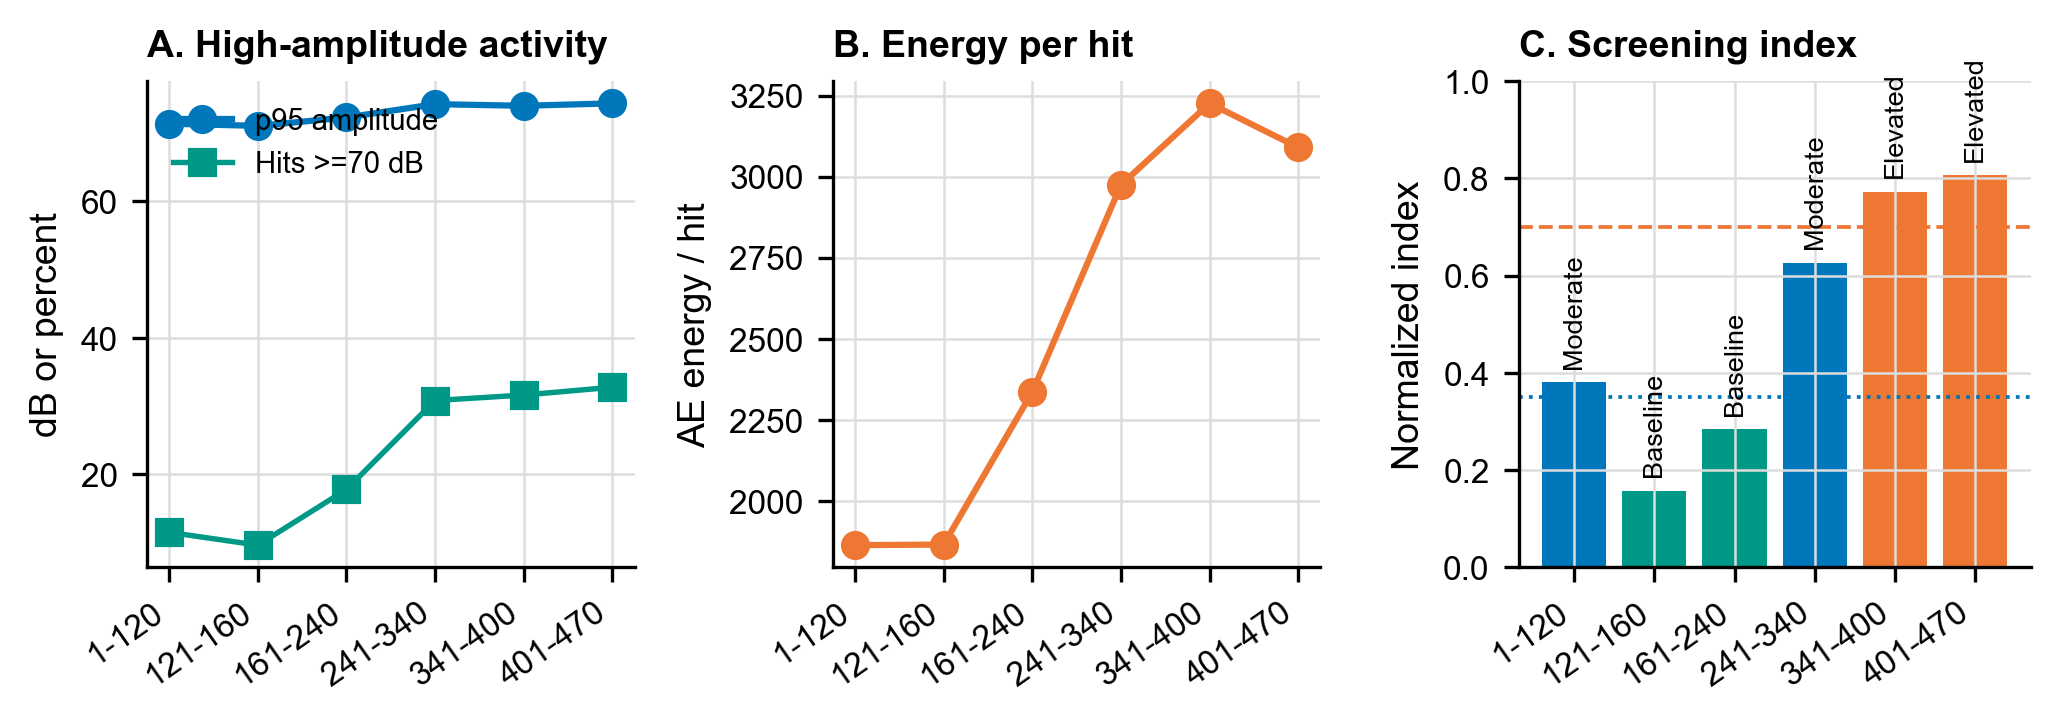
\includegraphics[width=\linewidth]{assets/fig04_ae_feature_monitoring.png}
\smallnote{Screening index ranks cycles 341--400 as the inspection-priority window.}

\vspace{0.6ex}
\metric{31.63\%}{records above 70 dB}
\hfill
\metric{$3.23\times10^3$}{energy per hit}
\hfill
\metric{125 kHz}{median frequency}
\hfill
\metric{1.17M}{feature records}

\vspace{0.7ex}
\begin{center}
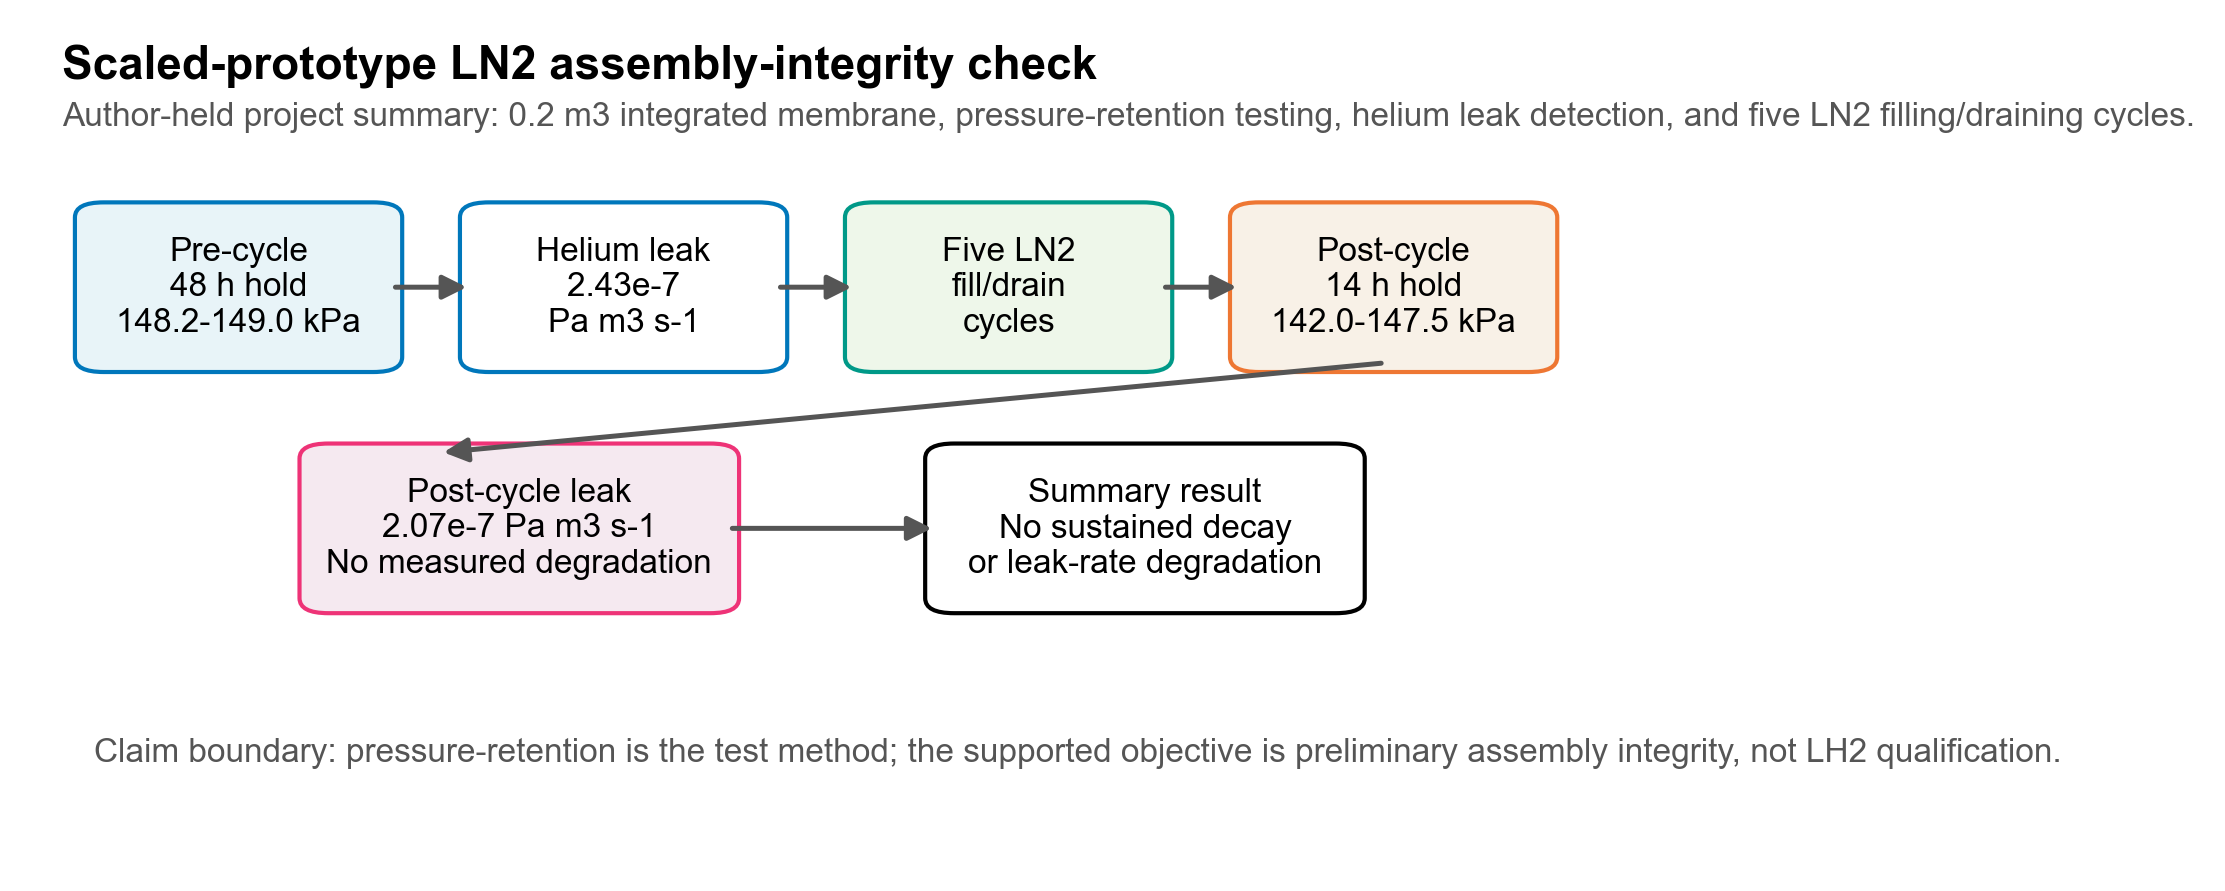
\includegraphics[width=\linewidth,height=17.2cm,keepaspectratio]{assets/fig05_ln2_integrity_gate.png}
\end{center}
\smallnote{Pressure-hold and helium leak-rate checks are the test method; the objective is to verify assembled-membrane integrity before and after five LN$_2$ filling/draining cycles.}

\compacttable
\renewcommand{\arraystretch}{1.10}
\begin{tabular}{@{}>{\bfseries}p{0.36\linewidth}p{0.52\linewidth}@{}}
\toprule
Check & Result \\
\midrule
Pre-cycle hold & 48 h at 148.2--149.0 kPa abs. \\
Post-cycle hold & 14 h at 142.0--147.5 kPa abs. \\
Pre-cycle leak & $2.43\times10^{-7}$ Pa m$^3$ s$^{-1}$ \\
Post-cycle leak & $2.07\times10^{-7}$ Pa m$^3$ s$^{-1}$ \\
\bottomrule
\end{tabular}
\end{posterblock}
